%KOKO
\documentclass[lang=cn]{elegantpaper}

\usepackage{array}
\usepackage{courier}
\usepackage{xcolor}
\usepackage{tabulary}
\usepackage{float}
\usepackage{makecell}
\usepackage{multirow}
\usepackage{zhnumber}

\title{智能手机传感器的现况与未来发展趋势}
\author{于海鑫 \\ 2017211305 班 \\ 2017211240}
\institute{北京邮电大学计算机学院}

\version{}
\date{\zhtoday}


% 本文档命令
\usepackage{array}
\newcommand{\ccr}[1]{\makecell{{\color{#1}\rule{1cm}{1cm}}}}

\begin{document}

\maketitle

\begin{abstract}
    随着时代的发展,智能手机逐渐成为了人们日常生活中的必须设备。现代的智能手机通常内置了高性能的微处理器以及一系列低成本的传感器,例如加速度传感器、GPS 传感器、数字指南针、甚至是超高清的相机。这一系列的传感器使得有需要的个人以及集体能够以较低的成本构建感知外部环境的程序。这些配备着低成本传感器的手机已经给诸多领域带来了革命性的变化。医疗保健、社交、交通优化等领域已经开始享受到了智能手机传感器带来的便利。本文我们将调研现有的手机传感器以及其应用。之后我们将着眼于智能手机内置的图像传感器、详细介绍其状况,同时我们将讨论未来传感器的发展趋势以及出现的新问题。
    \keywords{智能手机,传感器}
\end{abstract}

\section{引言}

现代智能手机通常配备有多任务式的操作系统,高性能的微处理器,种类丰富的低成本传感器以及无线联网基础。此类手机现在已经再全球范围内普及。

最早的将通话功能与计算功能结合在一起的设备大致可以追溯到上世纪的 70 年代。但是,直到上世纪的 90 年代,也就是 GSM 技术出现后,第一步商业化的移动电话才真正上市。当时可重复充电锂电池技术的出现进一步的拉低了手机的价格以及重量,使得其真正的成为了实用设备。最早出现的手机是 1992 年的 \emph{Nokia 1011},内置了一个麦克风作为传感器。在那之后,屏幕更好,续航更长,重量更轻、通信更快的手机逐渐出现。智能手机发展的一个里程碑是 2007 年 \emph{iPhone} 的出现:该设备内置了 2 MP 的相机、距离传感器、环境光传感器和加速度传感器。

当今的智能手机通常内置了种类繁多的传感器。大多数的设备都会提供高清相机、3轴加速度传感器、磁力传感器、麦克风、亮度传感器以及温度传感器。有些高端产品会内置更多的传感器:例如 Google 的 Nexus 5 内置了步数传感器、Samsung Galaxy 5S 内置了一个心率传感器、iPhone 8 Plus 内置了气压计等。

这些传感器的内置通常是为了支持一些功能。加速度传感器通常用来判断设备的方向,并允许屏幕方向随着设备旋转而进行切换。磁力计可以用于在指南针应用中检测北极的位置。温度传感器通常用来监测电池以及 CPU 的温度,防止过热损害设备。光传感器则会用来测量环境光的亮度,以自动调节屏幕的亮度。距离传感器用以检测设备是否在用户的耳边,以此可以提早关闭屏幕,防止通话时用户的耳朵进行了误操作。当然,除去这些在操作系统层面住哪被的功能外,用户也可以自行编撰程序,通过传感器的数据做一些工作。

本文中,我们将着眼于智能手机最常见的传感器 —— 图像传感器。在第二节我们将介绍图像传感器的构造。第三节将介绍图像传感器的详细应用。最后我们将对其未来应用进行展望。

\section{图像传感器:构造}

目前市场上主要有两种用于图像传感器的技术,即 CCD(电荷耦合器件)技术和CMOS(互补金属氧化物半导体)技术。两种技术的本质都是都将光线(光子)转换成电子信号(电子),其主要区别在于底层技术的设置。近年来,CMOS芯片技术已取得巨大进步,在多方面已超越CCD。凭借高速度(帧速率)、高分辨率(像素数)、低功耗以及最新改良的噪声指数、量子效率及色彩观念等各方面优势,CMOS芯片逐渐在CCD芯片主导的领域里占据了一席之地。当今的高端智能手机的图像传感器通常是基于 CMOS 技术的,因此,本文中主要讨论的是基于 CMOS 技术的传感器。

CMOS 图像传感器主要工作原理如图 ~\ref{fig:cmos}~ 所示,一系列光子打到像元(pixel)表面,光子被像元吸收后,激发产生一系列电子空穴对;电子被存储在电容上,转化为电压信号;电压信号经过一个模拟数字转化电路转换成电信号并输出。

\begin{figure}[H]
    \centering
    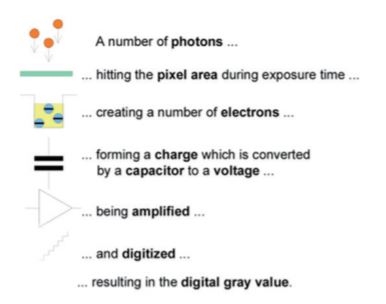
\includegraphics[width=.4\textwidth]{1-1.png}
    \caption{CMOS 原理}
    \label{fig:cmos}
\end{figure}

入射光透过微透镜、彩色滤镜和介质层到达硅片表面并被吸收,吸收的光子再转化为电子信号。其中,微透镜的主要作用是聚焦入射光,通过
微透镜可以增加入射到 PhotoDiode 表面的光。彩色滤镜的作用是为了滤除其他光波长的波,只通过绿色、蓝色、红色这三种波长光中的一种,其他光都滤除。在彩色滤镜中,通常使用的拜尔 Pattern,如图 ~\ref{fig:Pattern}~ 所示。可以看出其中绿色占一半,红蓝各占四分之一,这是因为人类视觉对绿光最敏感,使用两倍于红色或蓝色的绿色组件来模仿人眼的生理性质,我们将绿色光传感器称作光敏侦测组件,而红、蓝色则称为色敏侦测组件。最终每个像素点的颜色信息是经过插值处理得到的。

\begin{figure}[H]
    \centering
    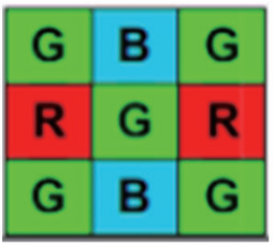
\includegraphics[width=.4\textwidth]{1-2.png}
    \caption{拜尔 Pattern}
    \label{fig:Pattern}
\end{figure}

可以发现,其内部的实现实际上是模拟了人眼感光的。

\section{图像传感器:应用}

图像传感器可以广泛用于自动阅读试纸。比色试纸被广泛应用于pH值的测量、尿液中病原体的检测、血液中葡萄糖水平的检测等操作中。将图像传感器应用于其上是很简单方便低成本的:只需将被测样品倒在试纸上,并等待色纸出现颜色变化。之后使用智能手机摄像头拍摄并分析颜色变化。这种应用的主要缺点环境光的干扰以及摄像头的不同对其准确度影响较大。为了克服这些问题,许多作者将智能手机临时放置在设计好的环境下并配备好固定的照明系统,以此滤除环境光的干扰,并配合软件校准算法以降低不同厂家的传感器之间的影响。

例如,S.D. Kim 等人在2017年提出了基于智能手机读取pH测试条的系统\cite{kim2017smartphone}:他们将手机放置在带有LED照明系统的3D结构内,使用纸质印刷参考色进行校准。 该系统已经过测试,平均误差低于0.25。


智能手机相机也可以用于测量紫外线辐射。众所周知长时间的暴露于紫外线辐射会增加皮肤癌的风险,因此,快速检测紫外线辐射的规模也是比较重要的主题。通常来说,智能手机的相机会带有一组滤镜,能去除掉不可见的波长,除此之外,相机镜头的图层也会吸收掉不少紫外线。但是,尽管如此,2013 年 Igoe 等人依然演示了如何在这种情况下检测 UVA 的波长\cite{igoe2013characterization}。这一实验已经先后在实验室模拟环境以及展示的室外环境进行了验证。后续该实验室还展示了使用智能手机检测 UVB 的波长的方式。上述的对于 UVB 的测量还可以用于评估大气中的臭氧总量\cite{igoe2018atmospheric}。除此之外,类似的技术也可以用于检测火山口的 SO2 排放强度\cite{wilkes2017low},不过需要外加的设备。

现代智能手机的普及使得便捷式计算机视觉应用得以发展。例如自动菌落的计数器,标准版计数是测量细菌浓度的一种参考技术。该技术该过程耗时且劳动密集。由于许多微生物实验室每天处理数百个板,每个板可包含数百个要计数的细胞,手动计数会导致眼睛疲劳出现差错。基于智能手机的自动菌落计数器利用手机摄像头获取培养皿的图片,然后将边界去除、图像平滑、图像二值化等操作用于图像,并计算菌落的数量\cite{minoi2016mobile}。

除此之外,图像传感器还可以用于检测心率等操作,更多应用受限于篇幅问题,不再详细叙述。

\section{图像传感器:未来}

随着现在智能手机发力于图像传感器以及整个相机体系,现在的旗舰手机的图像质量已经相比十年前有了长足的发展,甚至好于一些中小型相机的图像质量。在移动设备处理器性能明显过剩、专用处理器(例如 NPU)的移动化。曾经难以想象的需要高计算力的事情已经可以在手机上执行。在未来,更多的基于计算机视觉的应用会被发掘出来。同时基于图像传感器的 AR 或者 VR 技术在未来也会发挥出比较优秀的应用。

与此同时,我们不得不注意随着高像素带来的隐私相关的问题。例如之前所报道的,“剪刀手”照片通过照片放大技术和人工智能增强技术,就能将照片中人物的指纹信息还原出来。随着相机清晰度的大幅提升,此类隐私泄露的问题亟待解决。

\bibliographystyle{unsrt}
\bibliography{Ref}

\end{document}